\ChapterImageStar[cap:dar]{Análisis de Decisiones y Resolución}{./images/fondo.png}\label{cap:dar}
\mbox{}\\
\section{Metodología de evaluación}

La metodología de evaluación que se aplicó para la elección de la tecnología de Virtualización Basada en Contenedores (VBC) fue DAR (Decision, analysis and resolution) de CMMI \citep{CMMIInstitute2010}. Esta metodología permitió evaluar las necesidades del grupo GRID a través de un proceso estructurado que consideró múltiples alternativas, criterios de evaluación bien definidos y un análisis comparativo. En este caso, se identificaron y analizaron diversas tecnologías VBC —como Docker, Podman, LXC o Kata Containers— aplicando criterios como el tipo de licencia, la compatibilidad con herramientas de orquestación, el rendimiento entre otros. Mediante el uso de matrices DOFA, se logró visualizar las fortalezas y debilidades de cada opción, facilitando una selección alineada con los objetivos estratégicos del sistema. Así, el uso de DAR no solo aportó transparencia al proceso, sino también trazabilidad y justificación técnica frente a una decisión para la arquitectura de infraestructura basada en contenedores.

El proceso de evaluación quedó registrado en un vídeo explicativo disponible en \href{https://youtu.be/xOmuQs2RX2c}{link}.

\section{Resultados de la evaluación}

\begin{table}[H]
    \centering
    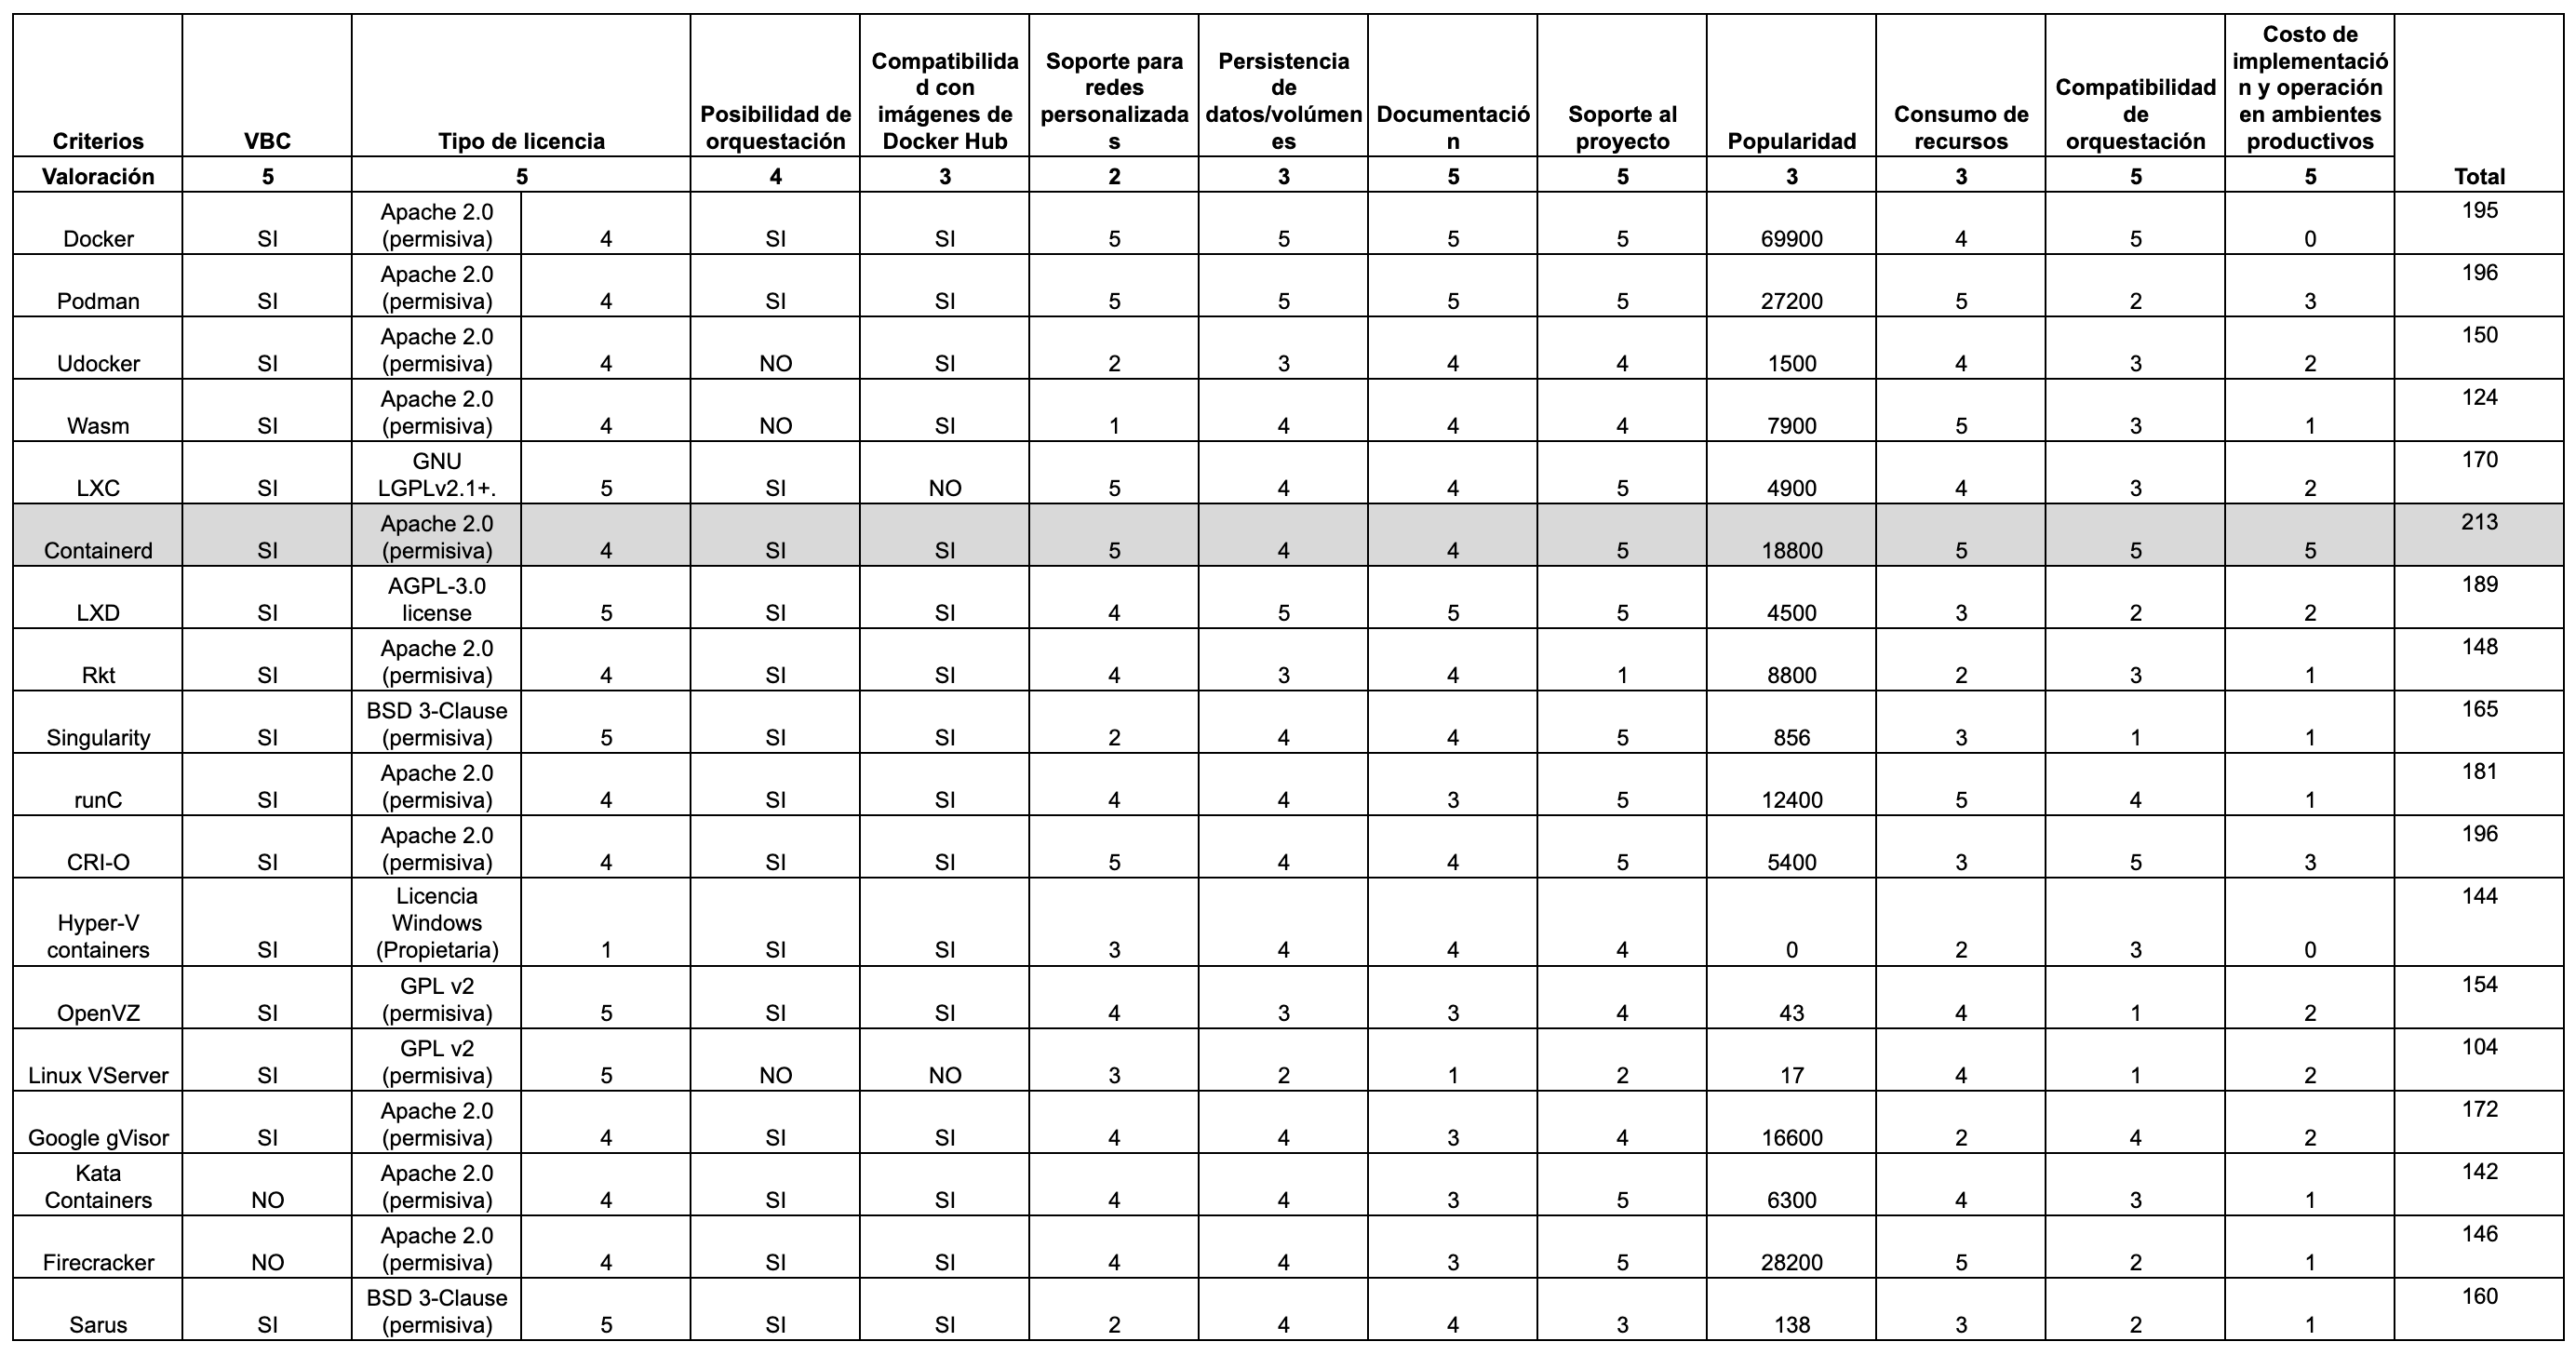
\includegraphics[width=\textwidth] {tablas-images/cp5/DAR.png}
    \caption{Análisis de Decisiones y Resolución (DAR) aplicado a la selección de VBC}\label{tab:tabla-dar}
\end{table}

\section{Criterios de evaluación}

\subsection{VBC (¿Es una tecnología basada en contenedores?)}
Este criterio define si la tecnología analizada entra dentro de la categoría de virtualización basada en contenedores, lo cual es el punto de partida para que pueda ser considerada en el análisis. Se evalúa como Sí (SI) o No (NO).

\subsection{Tipo de licencia}
Se analiza el tipo de licencia bajo la cual se distribuye la tecnología, ya que esto afecta su adopción en proyectos académicos o comerciales. Las licencias permisivas (como Apache 2.0 o BSD) permiten mayor libertad de uso y modificación, mientras que licencias restrictivas (como AGPL o licencias propietarias) imponen ciertas limitaciones legales o técnicas.

\subsection{Posibilidad de orquestación}
Se refiere a la capacidad de la tecnología para integrarse con herramientas de orquestación como Kubernetes, Docker Swarm o Nomad, lo cual es clave para la gestión automatizada de contenedores a gran escala. Una mayor puntuación indica mejor compatibilidad y soporte para estas herramientas.

\subsection{Compatibilidad con imágenes de Docker Hub}
Evalúa si la tecnología puede ejecutar imágenes obtenidas directamente desde Docker Hub, el repositorio más utilizado para contenedores. Esto facilita la reutilización de contenedores existentes y la integración con flujos de trabajo ya establecidos.

\subsection{Soporte para redes personalizadas}
Determina si la tecnología permite la creación y gestión de redes personalizadas entre contenedores. Este aspecto es fundamental en arquitecturas distribuidas, donde la comunicación entre servicios debe configurarse de forma segura.

\subsection{Persistencia de datos / volúmenes}
Analiza si la solución permite la persistencia de datos, es decir, que los datos generados dentro de un contenedor puedan mantenerse incluso después de reiniciarlo o eliminarlo. Esto se logra mediante el uso de volúmenes o sistemas de almacenamiento externos.

\subsection{Documentación}
Se valora la calidad, profundidad y accesibilidad de la documentación oficial. Una buena documentación facilita el aprendizaje, la resolución de problemas y la implementación efectiva de la tecnología.

\subsection{Soporte al proyecto}
Considera el respaldo que tiene la tecnología por parte de la comunidad, empresas o fundaciones (como CNCF o Red Hat). Esto incluye mantenimiento activo, actualizaciones regulares, y foros o canales de ayuda disponibles.

\subsection{Popularidad}
Este criterio mide la adopción y visibilidad de la tecnología, lo cual puede reflejar su madurez, confianza del mercado y disponibilidad de talento capacitado. Se puede estimar por métricas como el número de estrellas en GitHub.

\subsection{Consumo de recursos}
Evalúa el nivel de consumo de recursos respecto al uso de CPU, memoria y almacenamiento. Se valora según lo que mencionan las organizaciones en este aspecto.

\subsection{Compatibilidad de orquestación}
Difiere levemente del punto 4.3, ya que aquí se mide qué tan bien se integra con los orquestadores, considerando estabilidad, plugins nativos y experiencia de uso. Un puntaje alto indica integración fluida y confiable.

\subsection{Costo de implementación y operación en ambientes productivos}
Este criterio analiza los costos asociados a poner en marcha la tecnología en un entorno real. Incluye licencias, infraestructura, tiempo de configuración y mantenimiento. Una puntuación alta significa bajo costo o costo nulo, lo cual es ideal para instituciones académicas o proyectos con presupuesto limitado.

\section{Tecnología VBC ganadora}

Del análisis comparativo realizado, Containerd se posiciona como la tecnología de virtualización basada en contenedores con mejor desempeño general. Destaca por su alta compatibilidad con Docker Hub, soporte para redes y volúmenes, excelente integración con orquestadores como Kubernetes, y una licencia permisiva que facilita su adopción. Además, cuenta con una sólida documentación y un respaldo activo de la comunidad. Estas características hacen de Containerd la opción adecuada para ser implementada en ambientes productivos del grupo de investigación GRID, combinando los diferentes criterios definidos desde el grupo de investigación.

\section{Análisis DAR del motor de Kubernetes}

\begin{table}[H]
    \centering
    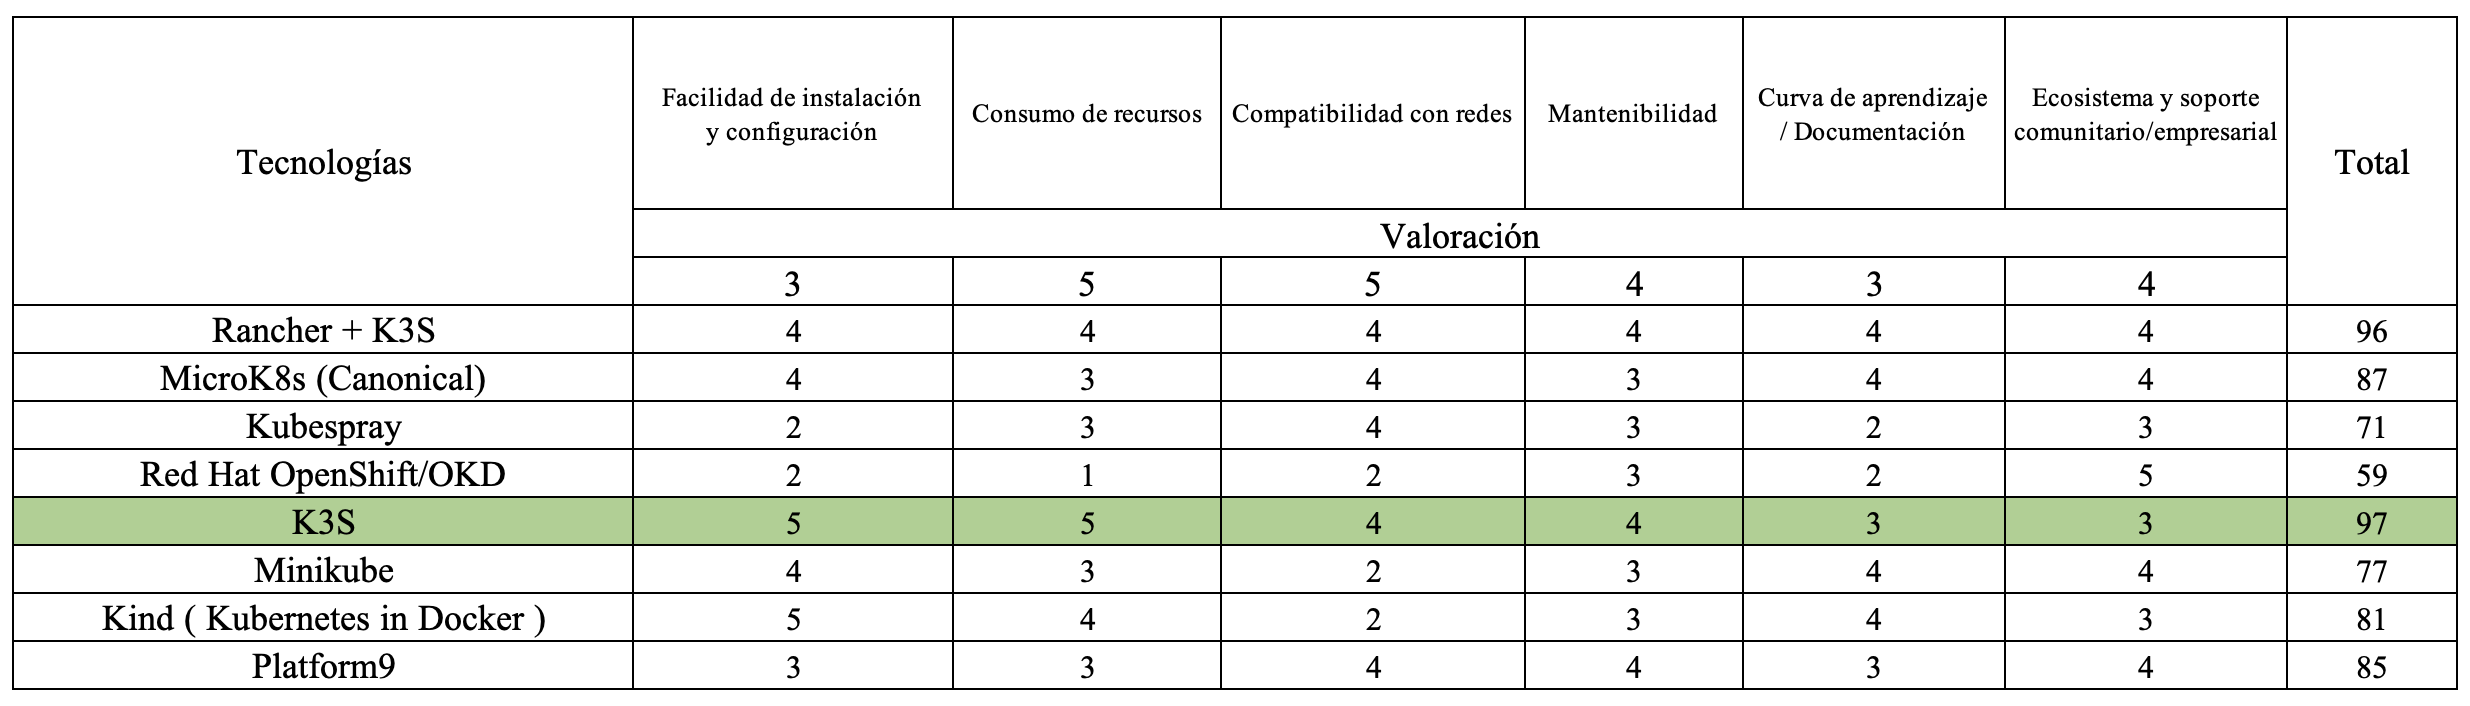
\includegraphics[width=\textwidth] {tablas-images/cp5/dar-k8s.png}
    \caption{Análisis de Decisiones y Resolución aplicado a la selección del motor de Kubernetes}\label{tab:tabla-dar}
\end{table}